\chapter{Jugements et Multi-dimensionnalité}
\label{chap:Jugements et Multi-dimensionnalité} %, indicateurs et interprétation} % lien de l'impact à la fonction entre inventaire et modélisation, déjà l'interprétation.
Au sein de la méthodologie et comme observé dans la revue critique de \citeauthor{reap_survey_2008}, un certain nombre de points sont des "décisions pivots".
Nous venons de faire la démonstration de la résolution de la problématique de la multifonctionnalité et nous affirmons qu'il en va de même sur l'ensemble des jugements dans la méthodologie.
Et puisqu'il s'agit d'observer l'ensemble des applications de jugements moraux au sein de la méthodologie pour corriger celle-ci, reprenons cette liste et traitons les, point par point, dans l'ordre méthodologique proposé en ISO et ILCD.
Sur cet ensemble, nous rechercherons les dimensions employées et leurs articulations entre les diverses questions.
À l'issue de ce déroulement, nous ferons la synthèse des dimensions et tenterons de proposer un ensemble cohérents de celles-ci sur lequel poser le jugement du décideur, l'\emph{interprétation finale}.

\section{Un ensemble de jugements}
%\colorbox{yellow}{avec ou sans le chapeau du chapitre ?}
%
%\colorbox{yellow}{intégrer Hafizan dans les applications (AHP sur les indicateurs)}

 \citeauthor{reap_survey_2008}, dans leur article, définissent les choix de l'exécutant comme décisions centrales (pivotal decisions, marqué d'un~"~a~" dans la table \ref{tab:PB non-resolus de l'ACV}).
 
!!!!!!!!!!!!!!!!!!!!!!!!!!!!!!!!!!!

 \colorbox{yellow}{check}
 
 reprendre table en fr pour reconstruire l'image
 
!!!!!!!!!!!!!!!!!!!!!!!!!!!!!!!!!!!
 
  \begin{figure}[h]
  %  \textwidth*0.5 : pas fonctionné
  %  figure à créer depuis le poster
    \centering
    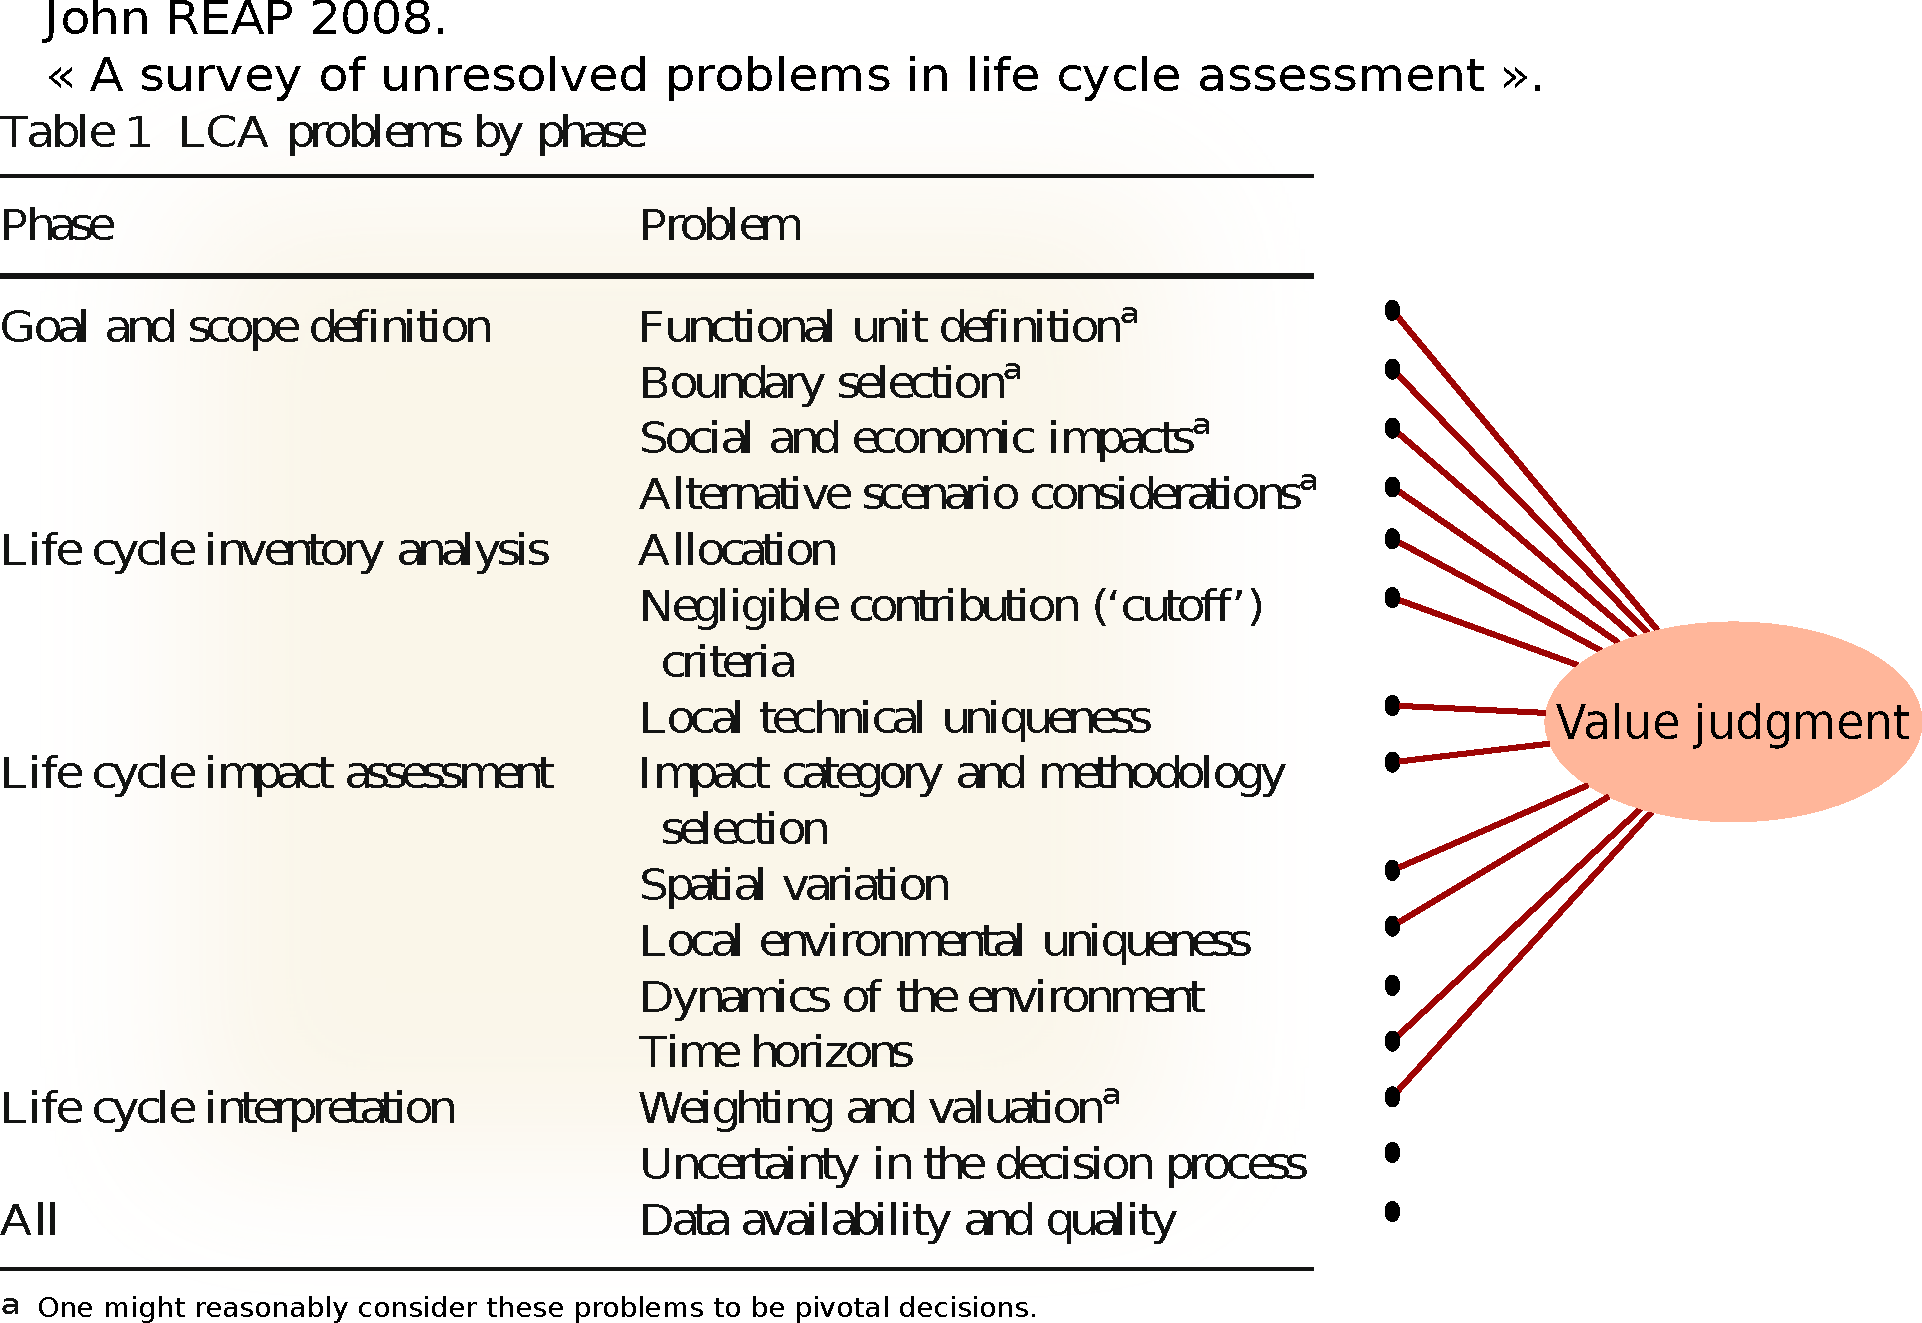
\includegraphics[width=\textwidth]{/home/rudy/Documents/rudy/01_These/11_production/01_COMMUNICATION/figures/value_quite_everywhere.pdf}
    \caption{Une multitude de jugements.}
    \label{fig:multitude_jugements}
  \end{figure}
Nous pouvons commenter le tableau~\ref{tab:PB non-resolus de l'ACV} en ajoutant que la sélection des méthodes et indicateurs d'impacts est également un choix du praticien.
Cette sélection peut s'apparenter à une pondération nulle des indicateurs existants mais qui n'ont pas été retenus dans l'étude.
De même les considérations qu'une différence temporelle, spatiale, technique, quantitative soit, ou non, négligeable ou non considérée est un jugement.
Comme nous venons de nous étendre sur la question de la multifonctionnalité, l'allocation relève tout autant de cette catégorisation.

Passons donc en revue chacune de ces questions.


%\subsection{How does the practitioner define the functional unit?}
\subsection{Définir l'unité fonctionnelle~?}

\exbox{
Un kilogramme de grain de blé pour produire de la farine n'est pas un kilogramme de grain de blé pour produire des pâtes (wheat grain, durum grain).
Nous tendons à réduire les entités aux attributs que nous connaissons à leur propos et plus encore à ceux que nous jugeons importants.
Nous oublions parfois que l'importance de la distinction entre des entités peut venir de la simple existence de la différence elle-même~\cite{corrado_new_2010}.
}

Pour dissocier ces produits similaires, il faut prendre en compte de plus nombreux attributs que la masse seule.
Ainsi, lorsque le praticien choisi l'unité fonctionnelle, il sélectionne relativement au produit observé ce qui selon \emph{lui} fait \emph{valeur}.
Donc, l'une des premières actions du praticien suivant les étapes de l'ISO ou de l'ILCD~\cite[]{european_commission_ilcd_2010}, ou du PEF~\cite{commission_europeenne_commission_2013}, est l'application d'un jugement de valeurs.
Il sélectionne les attributs et leurs combinaisons qui font sens relativement à sa propre perception de ceux-ci.
Pour prendre de la distance avec une perspective fonctionnaliste (nous rapprocher des systémistes), nous pouvons considérer que chaque flux apprécié comme fonctionnel est un flux portant des attributs que nous valorisons.
Nous pouvons donc dire que le système observé n'est pas un objet fonctionnel, mais simplement un système, avec des entrées et sorties en relation avec son environnement.
Ce faisant, nous reportons le jugement d'utilité, de fonctionnalité ou de valeur, au delà de la caractérisation objective.


%Example:
%
%One kilogram of flour grain to produce bread is not one kilogram of flour to produce pasta
%\footnote{We tend to reduce entities to the attributes we know about them and to those we consider ``important''.
%We some times neglect that some  entity we juge as a lesser one for its properties we judge at this time useful remain interesting and potentially important simply by its existence~\cite{corrado}}.
%To discriminate those similar products you have to take into account more numerous attributes than weight.
%\emph{So when the practitioner choose the functional unit, he's selecting what makes value to him.}
%So the first thing the practitioner do following ISO or ILCD\cite[]{european_commission_ilcd_2010} or PEF is making a value judgement.
%He selects the attributes and their combination that make sense according to his own perception of those attributes.
%To take distance with the functionalist perspective, we have to consider that the flow we consider functional are only flows with attribute we value.
%Then the system observed is not a \emph{functional } object, but rather an entity with input, output, in relations with its environment.
%And doing so we report the judgment of utility (or functionality), of value, outside of the characterization of the object (product or services).

%\subsection{How are selected boundaries?}
\subsection{Déterminer les frontières}
%\colorbox{yellow}{INSERT CRADLE|GATE|USE|GRAVE boundaries| si abs image libre, créer}

\textbf{Faut-il définir des frontières ou de définir des règles d'inclusion - exclusion~?}

Le périmètre est une conséquence directe de l'unité fonctionnelle.
Il s'agit de \textit{dé\textbf{finir}} (poser une fin) à ce qui contribue à la délivrance du flux de référence.
Cela concerne ce qui est appelé par certain praticien et chercheurs comme `premier plan'.
Ceci est repris dans l'ILCD.
\blockcquote[Figure 13, p., traduction]{europ}{
Représentation du système de premier plan et du système d'arrière-plan dans la perspective de la spécificité (voir encadré);
(À titre indicatif): Le système analysé a des limites (frontière en pointillés), la séparant du reste de la technosphère et de l'écosphère.
Le système peut être divisé en premier [et arrière] plan.
[Le premier plan est] le système des procédés qui sont spécifiques au système analysé, c'est-à-dire propres opérations et les fournisseurs fixes.
Les procédés dans le système d'arrière-plan ne sont pas spécifiques, mais acheté par l'intermédiaire d'un (théoriquement totalement homogène) marché.
Le système est la somme exacte de l'arrière-plan et des systèmes de premier plan.
Quantitativement flux non-pertinents peuvent être exclus, i.e. une coupure est pratiqué [cut-off] (flèches en pointillés).}
%Foreground system and background system in the specificity perspective (see box); (illustrative): The analysed system has boundaries (dashed border), separating it from the remainder of the technosphere and from the ecosphere. The system may be divided into the foreground system of processes that are specific to the analysed system i.e. own operations and fixed suppliers. The processes in the background system are not specific but purchased via a (theoretically fully homogenous) market. The system is the exact sum of the background and the foreground systems. Quantitatively irrelevant flows can be excluded, i.e. cut-off (dotted arrows).
%}
Cette contradiction méthodologique est le résultat des approches pré-informatique où il n'était pas envisageable de laisser numériquement converger un calcul puisqu'il était (et est toujours) réalisé par voie analytique et inverse de \textsc{Leontief}.

Dans les études de cas nous rencontrons différents types de frontières.
Des études sont définies `jusqu'à la~: porte, roue, tombe.
Il s'agit des expressions ``cradle to door'', ``cradle to wheel'', ``gradle to grave''.
\textbf{Elles renvoient à des évaluations ne tenant pas compte de la totalité du cycle de vie.}
Quelles sont les raisons légitimes pour ces divisions~?
Ne serait-ce pas une expression inadéquate de l'unité fonctionnelle et de sa présentation à une audience~?
Observe-t-on la production d'un matériau ou produit semi-fini, d'un carburant, ou d'usages~?
Si nous sommes confiants dans nos raisons pour approcher la problématique de l'évaluation environnementale avec l'angle holistique de la \emph{\textbf{globalité} du cycle de vie}, alors pourquoi ces divisions ?

Si les coupures de périmètre de cette nature sont courantes mais discutées, il est une coupure bien plus profonde.
Dans le jugement des ``flux non-pertinents'' qui ``peuvent être exclus'' se trouve une coupure toute particulière.
Il s'agit de la notre, celle envers l’être humain.
L'ACV ne tient pas compte des composants humains des rouages entrepreneuriaux.

%Is there a need to define boundaries or rather rules for inclusion?
%Is there a legitimate reason for those divisions, gate, wheel and so on?
%Or is it just a bad expression of functional units and their depictions toward audience?
%Do we look at the production of fuel or use of a fuel...?
%If we were confident in the need to address impact assessment for all life cycle due to report of the stage the impacts occurs, then why those divisions?
\exbox{
Lorsque nous cherchions les limites du cas d'étude de cette thèse, les opérateurs manipulant le produit ont été considérés.
Le produit est-il fonctionnel sans l'action de cette personne~?
Il s'agit ici d'une question totale.
Non-Oui, Oui, car sans lui pas de produit.
Exclure un composant essentiel du système productif serait loin d’être une coupure anodine et somme toute donc une erreur.
Si l'opérateur est un composant décisif du système observé, alors il est légitime de l'intégrer au périmètre du système.
Nous n'avons jamais observé d'étude ACV qui pourtant s'en préoccupe.

Il s'agit ici d'une entité hautement multifonctionnelle.
Faut-il l'inclure dans le système, lui \emph{et} le système qui l'a formé, éduqué, protégé, soigné, logé, nourri, diverti etc. ?
La personne est \emph{employée} sur une fraction de son temps, de vie, d'activité.
Une part du système lui permettant d'être fonctionnel dans son \emph{emploi} pourrait donc être allouée sur la base de cette fraction (temps d'emploi / temps éveillé).
\textbf{N'est-il pas incohérent d'observer l'ensemble du cycle de vie pour les entités matérielles et ne pas le faire parce qu'il s'agit d'êtres humains~?}
}
Cet exemple, peut-être jugé caricatural pour certains, aura le mérite d'exposer ouvertement l'étendue du système à observer  dans une approche holistique.
Nous avons choisi cet exemple à dessein.
Il souligne particulièrement les distinctions qui pourraient être faîtes entre des systèmes technico-sociaux ou \emph{une part non négligeable de ces fonctions est assurée hors marché}, par des mécanismes de socialisation, étatique ou non.
%When searching the limits of the case study I've been hired for, I considered the operators handling the product, focus of the study\footnote{What was I thinking, hum!}.
%Is the production functional without this person ?
%If the operator is a decisive component of the system I observed, then she/he is a legitimate part of it and the boundaries shall include the operator.
%Be damed this component is highly multi-functional\footnote{I was sure it was gonna trouble me! I should stop thinking. This delays the deliverable way too much!}!
%Should I include part of the system that feeds her/him, that educated-s him/her, that protects, houses, heals, entertains her/him ... ?

Ainsi, déclarer l'importance du set de fonctions observées (considérées en services ou produits), est un choix de déclaration de valeurs envers un but perçu.
Le périmètre est la seconde étape respectivement à l'ISO.
Une nouvelle fois il s'agit, comme pour l'unité fonctionnelle, de l'application d'un jugement de valeur.

%So stating the importance to the set of function(s) observed (considered as services or products), is a choice of declaring the value toward a perceived goal.
%It is the second thing done according to LCA's guidelines and standards.
%It's still the same matters discussed for functional definition.
%It is still the elicitation of values and preferences.

%\subsection{What is considered negligible?}
\subsection{Considérer comme négligeable}
Sous ce thème je considère diverses formes de coupures (hors questions de périmètre).
Les originalités, techniques, spatiales, temporelles, environnementales, au sens ou elles sont des coupures qualitatives, comme les coupures quantitatives, ne doivent pas être traitées isolément.


%Under this question I consider all Cut-offs.
%Are uniquenesses negligible, ``Local technical uniqueness'', ``Spatial variation'', ``Local environmental uniqueness''?
%In the sense they are cut-offs of qualitative nature when cut-off usually addresses quantification.
%It is the same issue to me and cannot be divided in my opinion.
\exbox{
Posons-nous dans l'ordre les questions suivantes~:
\begin{enumerate}[noitemsep,topsep=0pt,parsep=0pt,partopsep=0pt]
 \item Combien de temps de votre vie considéreriez vous comme une coupure acceptable (cut-off)~?
 \item Combien de centimes de votre salaire considéreriez vous comme 'jetables'~?
 \item Quelle quantité alimentaire avez-vous laissé dans votre assiette lors de votre dernier repas~?
 \item Aviez vous préparé ce plat, attendu dans une file pour l'obtenir, payé pour qu'il soit devant vous dans cette assiette~?
\end{enumerate}
Ressentez-vous poindre lors de la question (4) l'inconsistance des réponses spontanément formulées entre (3) et (1+2).
%How much time of you life would you consider to acceptably cut-off?
%How many cent of you wages would you consider disposable off?
%How much food did you left to garbage in the plate of your last meal even-though you cooked it, waited in a queue for it or bought it?
}

Commençons par interroger la coupure quantitative.
En mécanique, certains matériaux sont caractérisés par leur résistance élastique.
Mais tous les matériaux ne présentent pas de palier pour distinguer un domaine plastique.
Un seuil arbitraire est alors définit (en \% d'allongement).
Ceci est fait parce qu'il n'y a pas de signe de convergence apparent sur une valeur à la frontière des domaines plastique et élastique.
Lorsqu'une courbe converge, la grandeur qui retient notre attention est la limite vers laquelle elle tend.
Ainsi, plus qu'un critère arbitraire de coupure quantitatif, ne devrions nous pas proposer une valeur de convergence de l'inventaire~\barre{?}~!
 
%In mechanic, some material are characterized by elastic strength.
%But not all material (particularly ductile one) have a yield stress to identify plastic domain precisely.
%The yield strength is then defined by an arbitrary off-set.
%This is done because there is no sign of convergence on some value to depict the frontier between plastic and elastic domains.
%When considering a convergent curve, by expressing a model of this curve, the convergence limit can be calculated.
%So more than the cut-off of LCI, shouldn't we propose a converged value of LCI?

Traitons maintenant la question qualitative.
Tant que nous disposons d'une information spécifique, pourquoi n'en ferions nous pas usage~?
L'agrégation des informations spécifiques suivant diverses classifications n'en sera pas moins exploitable lorsque l'utilisateur ne sera pas en mesure de préciser sa spécificité.
L'influence d'une application de données agrégées sous des catégories plus ou moins grandes sera sur la forme des fonctions de préférence sur les outils de surclassement cf~\ref{sec:ADMC}.

%As long as we have specific information, accordingly with restrained variability, I don't see a reason for not using it.
%The generic data still hold its variability and uncertainty.
%Either generic or not, they characterize the same object and using dissimilarly specialized data only interact with the preference form to consider when opposing the distributions.

%\colorbox{yellow}{GRAPH boxplot réduite et large. Pourquoi pas l'article sur les éoliennes de l'école BLANC}.
Actuellement au sein de l'ILCD, comme discuté par Lynda \textsc{Aissani}\footnote{Lors d'une formation EcoSD.}, l'utilisation de données spécifiques (non-génériques) "doit être justifiée"~\cite[Provisions: 6.7]{european_commission_ilcd_2010}
~\footnote{\blockcquote[Provisions: 6.7]{european_commission_ilcd_2010}{
XI) OBLIGATOIRE - Lieu et heure \textbf{méthodes d'AICV non génériques}: L'\textbf{utilisation} potentielle de méthodes d'AICV qui ont été dérivées des originales, celles comportant les localisations génériques et temporalités génériques (c-à-dire qui ne soient pas génériques, mais par exemple, spatialement ou autrement plus différenciées ou modifiées) \textbf{doit être justifiée} relativement à l'objectif et la portée de l'étude.
%XI) SHALL - Location and time \textbf{non-generic LCIA methods}: The potential \textbf{use} of LCIA methods that have been derived from the original, location-generic and time-generic ones (i.e. being not generic but e.g. spatially or otherwise further differentiated or modified) \textbf{shall be justified} along the goal and scope of the study.
}}
, alors que l'utilisation de données génériques, même si moins appropriées, n'implique pas cette justification.
%Currently within ILCD, as exposed by Lynda XXXXXX during EcodSD training, the use of specific methods ``shall be justified''\cite[Provisions: 6.7]{ilcd} when using generic even-though not the most appropriate is accepted without this justification.
Juridiquement nous dirions que la \emph{charge de la preuve est inégalement répartie suivant les défendeurs}.
C'est une problématique récurrente en science et en argumentation de façon générale\footnote{À titre d'exemple~:
\blockcquote{deshpande_signification_2011}{
[\ldots] la charge de la preuve est inégalement répartie
entre les deux camps.
\textbf{Les tenants d’une rupture avec le statu quo doivent être beaucoup plus convaincants que ceux qui se satisfont
de la situation actuelle.}
}
}.
Lors de l'application d'une orthodoxie, une vérité populaire, la vigilance scientifique ou critique chute. % (retrouver l'article de socio XXX ref). %\footnote{application marketing et cinématographique, les rire et applaudissement dans une série "comique"}.
%In law I would say the burden of the proof is unequally establish according to the defendants.
%We find here a recurrent issue of many sciences.
%When using orthodoxies, popular beliefs scientific vigilance drops\footnote{It works with all kind of vigilance. Citizens are also regularly fed with already accepted messages. This is interestingly developed in \citeauthor{} ?? bourdieux ? retrouver la video d'USUL et la source.}.
Il ne s'agit pas ici de dire que les hétérodoxes ne devraient pas avoir à se justifier.
Nous disons simplement que les orthodoxes le devraient également.
%It is not that heterodox should not justify themselves.
%It is that orthodox should too.

Sur un point plus spécifique, nous souhaitons également mentionner la différenciation des comportements normaux, anormaux et accidentels des systèmes étudiés.
L'article de \citeauthor{plumblee_marlos_2014} sur l'intégration des risques et événements non-ordinaires de la vie d'un produit montre les coupures que nous faisons sur les scénarios de vie considérés~\cite{plumblee_marlos_2014}.
L'intégration des données `qualité' et fiabilité (temps moyen entre deux défauts MTBF, qualification des défectuosités\ldots) pourrait tout à fait compléter nos modèles de descriptions.
L'intégration des questions de coût (LCC) le nécessiterait d'ailleurs pour plus de cohérence avec les charges d'assurances.
Il y a donc encore des corrections méthodologiques à apporter à l'ACV décrite dans les référentiels sur ce point.
%\footnote{
\exbox{
\blockcquote[traduction]{european_commission_ilcd_2010}{
Dispositions: 6.7 Préparation de la base d'évaluation d'impacts III.e)
Ils sont liés exclusivement aux flux élémentaires
(à savoir les interventions entre la technosphère et l'écosphère)
pendant des conditions de fonctionnement normales et anormales,
mais \textbf{excluant les accidents, les déversements et autres.} [ISO!]
%Provisions: 6.7 Preparing the basis for the impact assessment III.e)
%They shall be related exclusively to elementary flows
%(i.e. interventions between the technosphere and the ecosphere)
%during normal and abnormal operating conditions,
%but \textbf{excluding accidents, spills, and the like.} [ISO!]
}
}
%On a specific point I'd like to stress out a particular point on a qualitative cut-off, that is normal and ab-normal behavior of the studied system.
%It is defined in

Maintenons notre analyse des occurrences des jugements de valeurs dans la méthodologie.
Là encore, la détermination du périmètre en use sous de multiples orientations.
%But to remain in our list of modeling choices, again cut-offs are the judgment of importance (value) of additional data.
%And rules about cut-offs are questions of preference forms, i.e. how we value the difference between sets of data.
Sur le caractère quantitatif nous retiendrons, lorsque cela est possible, la recherche de la quantité `convergée' plutôt qu'une troncature d'une quantité déjà partielle.
Sur le caractère \emph{quali}tatif, nous retiendrons qu'il faut exclure l'exclusion méthodologique.
Ceci implique de pouvoir former à loisir sur la base des \emph{quali}fications des catégorisations pour l'accessibilité cognitive des parties-prenantes.
%\subsection{How should we consider time?} 
\subsection{Considérer le temps}
\label{subsec:Considérer le temps}
Sont incluses sous cette interrogation, la ``considération de scénarios alternatifs''
\footnote{
Ici, il s'agit des projections futures sur le système modélisé~\cite{reap_survey_2008}.
Elles impliquent des projections statistiques actuelles, mais aussi une orientation de 'où la société devrait-elle aller~?', aux travers des actions modifiant le "cap actuel".
},
l'"Environnement dynamique" et l'"horizon temporel".
Ces thèmes sont de même nature et traitent de notre rapport au temps, future mais aussi passé.
\citeauthor{murray_transdisciplinary_2015} rapporte les éléments suivants.

\blockcquote[traduction]{murray_transdisciplinary_2015}{
Hertwich et al. (2000)~\cite{hertwich_theoretical_2000} considèrent l'effet des valeurs dans la caractérisation telle que sur le potentiel de réchauffement climatique et l'actualisation des impacts futurs.}
Plus particulièrement \citeauthor{hertwich_theoretical_2000} font la critique de l'interprétation commune de la
\blockcquote[traduction]{hertwich_theoretical_2000}{
%According to a common interpretation, the
norme internationale sur l'ACV qui exige que les méthodes d'évaluation utilisées dans les comparaisons publiées soient ``libre de valeur''.
%international standard on LCIA requires that the assessment methods used in published comparisons be “value free.”
}
\keybox{
Nous retrouvons pour le temps comme tout autre dimension l'inséparabilité de l'é\textbf{valuation} et des \textbf{valeurs}.
}

\blockcquote[traduction]{murray_transdisciplinary_2015}{
Hellweg et al. (2003) examinent des raisons économiques pour l'actualisation et concluent que l'actualisation basée sur les «préférences temporelles pures» ne doivent pas être appliquées dans l'ACV pour des raisons éthiques.
}
Ceci souligne l’inconsistance propre à la vision courte de l'individu isolé.
\keybox{
Nous pourrions \emph{vouloir ne pas juger} du futur ou du passer, que nous ne pourrions pas.
Même considérer l'égalité de traitement sur l'ensemble de l'horizon temporel serait en fait un jugement.
}

Dans l'analyse de \textsc{Hellweg},
\blockcquote[traduction]{murray_transdisciplinary_2015}{
le type d'éthique n'est pas spécifié, mais semble être lié à la notion d'équité entre les générations.
Néanmoins, il est reconnu que les décideurs utilisent souvent des taux d'actualisation sur la base de préférence pure (définie par Hellweg comme «impatience»).
Hellweg et al. (2003) notent également que toute application d'une «valeur actualisée» pour les flux physiques suppose la \textbf{monétisation} et une série d'autres conditions telles que la \textbf{compensation} des générations futures et une approche de l'incertitude.
Le type de décideur et de leurs objectifs affectera également le choix du taux d'actualisation
(caractérisée par le taux de réduction privé ou social).
%Hertwich et al. (2000) consider the effect of values in characterisation such as global warming potentials and the discounting of future impacts.
%Hellweg et al. (2003) review economic reasons for discounting and conclude that discounting based on ‘pure time preferences’ should not be applied in LCA for ethical reasons.
%The type of ethics is not specified but appears to be connected to the notion of inter-generational equity.
%Nonetheless, it is acknowledged that decision makers often use discount rates based on pure time preference (defined by Hellweg as ‘impatience’).
%Hellweg et al. (2003) also note that any application of a ‘time cost of money’ to physical flows assumes monetisation and a range of other conditions such as compensation of future generations and an approach to uncertainty.
%The type of decision maker and their goals will also affect the choice of discount rate
%(typified by the private or social discount rate).
}
\keybox{
Nous voyons donc une domination de la discipline par un mode de pensée économico-monétaire chevillé à la substituabilité (généralisation du caractère compensable des choses).
C'est à dire que la discipline reconnaît ici sont échec face à la multi-dimensionnalité.
}
%I consider ``Alternative scenario considerations'' \footnote{here scenario considerations are future projection of the modeled system~\cite{reap_survey_2008}.
%They imply statistical projections, current state but should also integrate a Where does society want to go.},  ``Dynamics of the environment'' and  ``Time horizons'' to be of same nature, being the importance granted to future.


Il y a des inconsistances dans l'emploi disjoint de jugements de valeurs à travers les diverses étapes de l'ACV et la question de l'horizon temporel en offre un particulier.
%There are inconsistencies when not considering the value system for all the LCA steps, and ``Time horizons'' give us a good example.
Nous allons considérer les recommandations ILCD sur les méthodes d'impacts.
%On this case we will consider the ILCD recommendations.
Les méthodes d'impacts considèrent généralement trois horizons temporels issus des archétypes développés pour ECO-98.
Il s'agit des horizons à 20, 100 et 500 ans.
La recommandation par défaut est de 100 ans pour l'ILCD (3.1.6 Recommended default method at midpoint level)~\cite{jrc_ilcd_2011}.
Le manuel indique aussi la nécessité d'une représentativité temporelle correcte~\cite[6.8.4 Time-related representativeness]{european_commission_ilcd_2010}
%Impact methods consider three time horizons, 20, 100 and 500 years methods~\cite{jrc_ilcd_2011}.
%The guidance indicate the need for time representativeness \cite[6.8.4 Time-related representativeness]{european_commission_ilcd_2010}
\blockcquote{european_commission_ilcd_2010}{I) OBLIGATION - Bonne représentativité temporelle~: L'inventaire dans son ensemble doit avoir une représentativité temporelle aussi bonne que requise, en accord avec le but de l'étude.}
%\blockcquote{european_commission_ilcd_2010}{I) SHALL - Good time-related representativeness: The overall inventory data shall have an as good as required time-related representativeness, according to the goal of the study (see the accuracy requirements identified in chapter 6.9.2)}

Puis dans la procédure d'allocation décrite pour les co-produits, la formule est développée sur la fraction recyclée sans dépendance à l'échelle temporelle.
\exbox{
%In the allocation procedure described for co-product, the formula developed consider recycled fraction and process without time dependence.
% The allocation of the ``two steps allocation procedure'' lies in three part\footnote{I'm not kidding. Its juste the detailed three parts of the second step.}
%   \begin{enumerate}
%    \item Determination of the total use.
%    \item Sum of inventories of total use.
%    \item Mean of the previous sum.
%   \end{enumerate}
%   
%   ~\\
%   The total use quantity:~U
%   \footnote{
%   This is the result of geometrical progression of recycling a fraction of initial product (p) by a recycling rate (r).\\  
%   $u_2$ is the material quantity used after two recycling. $u_2= p+p*r+p*r^2$~\\
%   With $1+r+r^2+...+r^{n} = \frac{1-r^{n+1}}{1-r}$~\\
%   proof~:
% 
% \[ \left.
%     \begin{array}{rlcll} 
% 	Sn= &1&+&r+r^2+...+r^{n}& \\
%       r*Sn= &&&r+r^2+...+r^{n}&+r^{n+1}\\
%     \hline
%     Sn-rSn= & 1 && & -r^{n+1}\\
%     \end{array} 
%   \right. \]
%   $Sn=\frac{1-r^{n+1}}{1-r}$.}
% u'
% p
% r
% total amount of uses after first and second recycling loop
% primary amount
% average recycling rate [0...1), incorporating both collection efficiencies and processing
% efficiencies
% U
%  total amount of use
% i
%  recycling loop number
% n
%  total number of recycling loops
% 
   \begin{itemize}
    \item U~: quantité d'utilisation totale.
    \item i~: la boucle de recyclage.
    \item n~: le nombre de boucles de recyclage.
    \item r~: le taux moyen de recyclage, incluant à la fois la collecte et la transformation.
    \item p~: la quantité initialement produite.
   \end{itemize}
%   ~\\
   \begin{equation}
   U = \sum_{i=1}^{n}p*r^i=p*\frac{1-r^{n+1}}{1-r}
   \end{equation}
%   ~\\
%   ~\\
   L'inventaire du cycle de vie (ICV) de la quantité d'utilisation totale~:~I
   \begin{itemize}
    \item I~: ICV total d'une unité de produit (matière, pièce, vecteur d'énergie). % confirmer le terme, source, vecteur
    \item P~: ICV de la production par unité de produit.
    \item R~: ICV de l'effort de réutilisation, recyclage, revalorisation par unité de produit.
   \end{itemize}

L'inventaire complet suit la formulation~:
%The complete inventory I, is formulated as:
  \begin{equation}
   I = p*(P+W+R*\frac{r-r^{n+1}}{1-r})
  \end{equation}
%   Suivant le développement ci-dessous~:~\\
%   \[U=p+p*r+p*r^2+ ... +p^n\]~\\
%   \[U=p*(1+r+r^2+...+r^n)\]~\\
%   \[U=p+ \overbrace{p*r*(1 +r+r^2+...+r^{n-1})}^\text{Fraction réutilisée, recyclée, revalorisée, {\bf produite}}\]~\\
%   Il est important ici de comprendre la quantité à l'issue de l'effort R comme la quantité produite et non pas la quantité traitée !
%   
%The total use of the extracted material is developed as:
%  \begin{equation}
%  U = \sum_{i=1}^{n}p*r^i=p*\frac{1-r^{n+1}}{1-r}
%  \end{equation}
   Inventaire moyen d'une unité de produit~:~e
%The mean inventory is developed as
  \begin{equation}
  e= \frac{I}{U}=\frac{p*(P+W+R*\frac{r-r^{n+1}}{1-r})}{p*\frac{1-r^{n+1}}{1-r}}
  \end{equation}
%   
L'ILCD donne ensuite le raisonnement aux limites tel que~:
%With the consideration of ``infinite number of loops''\cite[Two steps allocation procedure, eq. 12]{jrc_ilcd_2010} in ILCD's guidance the share of inventory for waste treatment and primary production in the resulting average LCI/kg is only of the non-recycled part.
%And ILCD's guidance gives reasoning to limits as:
  \begin{equation}
  e=(P+W)*(1-r)+R*r 
  \end{equation}

Ceci peut être décrit de la façon suivante~:
En moyenne sur la somme des utilisations, les efforts de production primaire et de traitement des déchets (ultimes) ne sont comptabilisés que pour la fraction qui ne sera pas recyclée.
La production primaire et le traitement du déchet final sont très dilués par le cumul d'utilisation du recyclage
   \footnote{
   Le manuel rappelle que ce raisonnement suppose une égalité technique entre le bien primaire et le secondaire (recyclé, réutilisé ...).
   L'écart éventuel d'une génération sur l'autre doit être corrigé par un facteur
   \cite[14.4.1.2. Annexe C : modélisation de la réutilisation, du recyclage et de la valorisation énergétique]{european_commission_ilcd_2010}.
   Traduit de la version anglaise~:
   \blockcquote{european_commission_ilcd_2010}{Ce facteur de correction devrait être le ratio de prix de marché du produit secondaire sur primaire.}
   }
\keybox{
   Ce guide suit donc une logique de substituabilité marchande monétaire dont il ne semble capable de se défaire.
   }
   
   REPRENDRE LA TRADUCTION ou citation de la section ilcd et des equations correspondantes.
}
Pour ceux faisant l'effort d'appliquer la formule développée sans un nombre \emph{infini} de boucles, la \acrlong{MFA} nous montrera que certains secteurs peuvent 'stocker' la matière sur une durée importante (construction en tête sur plusieurs dizaines d'année)~\cite{davis_time-dependent_2007}\footnote{\citetitle{davis_time-dependent_2007}}.
Ce stockage souligne le délai temporel aux flux suivants (élémentaires comme produits).

And for those making the efforts of using the developed formula without this infinite number of loops [formula 11], MFA analysis shows us that may steel consuming sector is building and the good produced have long lifetime.

Accorder une part d'inventaire pour la fraction de matière qui sera potentiellement ré-employée dans une ou plusieurs centaines d'années et ne pas prendre en compte que l'activité extractrice a déjà eu lieu, ou est en cours, semble être un manque important de représentativité temporelle.
Granting a share of the inventory to a fraction of the material re-used in one hundred year from now and not take into account that extracting it was putting the burden on the environment \emph{now} is a serious lack of time representativeness to me.

De plus, il ne peut être déterminé aujourd'hui la quantité de ce qui sera recyclé aux taux et techniques actuelles ou à des taux spéculatifs ultérieurs.
Les suppositions et hypothèses des projections dépendent des jugements et des orientations que l'on souhaite pour le futur.
How much of what will be recycled can really be addressed by current rates of recycling, consumption and emission?
Quelles est alors la part effectivement recyclée dans l'horizon temporel sélectionné~?
What share is indeed recycled within the time horizon selected?
Ceci nécessite l'intégration des données de durée des procédés dans les descriptions de procédés et systèmes.
La dimension temporelle n'est-elle de toute façon pas nécessaire au traitement de la question des concentrations des substances émises~\barre{?}~!
According to the time horizons selection shouldn't we integrate lifetimes of products and lead-time production of processes?
Isn't the time dimension necessary anyway to address concentrations issues of all the substances handled?

Ici encore, sur plusieurs points nous avons vu l'importance de la considération du temps, de façon consistante, pour nous et les générations futures.
Here on several points, is considered value and relevance of time, ours and that of future generations, humans or else.
By not singling out the value system at play, the current methodology is inconsistent.

La perspective temporelle porte aussi une signification spécifique à un outil tel que l'ACV.
La modélisation du système vise aussi la localisation temporelle des choses changées suivant les alternatives.
Devrions nous considérer les alternatives pour les dommages passés ou futures~?
Si nous accordons toute l'importance au futur, rejetant de considérer un passé sans levier d'action actuel, allons nous générer une rétroaction permettant à une situation passée de se reproduire.
Sur quelle durée considérer l'influence de cette rétroaction, quand y-a-t-il prescription~?
Il faut donc déterminer un horizon temporel amont et un horizon temporel aval.
Concernant l'amont, il s'agit (au moins pour partie) de données objectives sur l’observation des rétroactions d'une production non-écoulée.
Time perspective also bears a specific topic for a decision tool such as LCA.
Modelling a system is also defining when (on top of where) things are changed.
Should I reconsider a choice of alternative for paste damage or incoming and future ones?
I chose to grant weight to future impacts considering that what matter is changing future emission, not those already made that I cannot change.
But granting positive feedback by consuming products responsible for these emission trigger their renewal.
So how long is this delay of past emission triggering negative feedback?
When start the environmental prescription to engage an alternative future?

% %!!! Keybox pb

\keybox{
Une part de cette dimension doit donc être traitée à la fois dans le domaine objectif et dans le subjectif.
\begin{itemize}
\item Le décideur considère comme important une plage temporel.
\item Un espace temporel objectif affecte l'espace subjectivement important.
\end{itemize}
Sans les lumières des sciences, point de rationalité consistante pour les jugements sur cette dimension.
}
%
%%\subsection{How should we value thing?}
%\subsection{Valoriser et apprécier les choses}
%La valorisation et l'appréciation englobent diverses interrogations.
%Nous regroupons ici les questions de "Pondération et évaluation", "Allocation" et "Sélection d'impacts".
%%Stated as ``Weighting and valuation'', ``Allocation'' and ``Impacts SelectionS''.
%Nous considérons la "Sélection des impacts sociaux et économiques " et la "Sélection des catégories et méthodes d'impacts " comme relevant du même thème, de la détermination des indicateurs observés, de la recherche de 'ce qui fait valeur'.
%%I consider ``Social and economic impacts selection'' as well as ``Impact category and methodology selection'' to be of the same nature of defining attributes of interest and the way to grant them value.
%
%Comme illustré pour l'unité fonctionnelle, le périmètre, l'appréciation des variations spatiales et temporelles, le problème est un tout portant sur l'attribution de la valeur au sein du système modélisé pour le décideur.
%Ceci peut être considéré comme le défaut centrale de l'\gls{ACV} dans sa méthodologie actuelle.
%
%%I kept this one to be the last but not the least.
%%As specifically illustrated for functional unit, boundaries or appreciation of time and spatial dimensions, the whole problem is to give value to attributes of the modeled system.
%%It can be considered the central lack within LCA's methodology to be corrected.
%
%Comme nous l'avions souligné pour la question du temps,
%les normes et manuels indiquent par exemple qu'il ne faut pas pondérer pour des assertions comparatives.
%Nous soulignons l'incohérence de l'ISO comme de l'ILCD par l'extrait suivant. 
%%\footnote{
%\exbox{
%\blockcquote[traduction]{european_commission_ilcd_2010}{
%5.2.5 Les comparaisons destinés à être divulgués au public
%(Fait référence à l'aspect de la norme ISO 14044: 2006 chapitre 4.2.2)
%[\ldots]
%Notez que, également selon la norme ISO 14044: 2006, une étude d'ICV seule ne doit pas être utilisée pour les assertions comparatives destinées à être divulguée au public, à savoir une évaluation de l'impact du cycle de vie et de \emph{l'évaluation} / interprétation \emph{doit être effectuée également}.
%}
%[\ldots]
%\blockcquote[traduction de la Dispositions: 6.7 Préparation de la base de l'évaluation de l'impact]{european_commission_ilcd_2010}{
%Normalisation et pondération: [\ldots]
%Notez que si l'étude comprend une assertion comparative devant être divulguée au public, \emph{la \textbf{pondération} quantitative des résultats des indicateurs publiés est \textbf{interdite}.
%}
%5.2.5 Comparisons intended to be disclosed to the public
%(Refers to aspect of ISO 14044:2006 chapter 4.2.2)
%
%Note that, also according to ISO 14044:2006, an LCI study alone shall not be used for comparative assertions intended to be disclosed to the public, i.e. a life cycle impact assessment and evaluation / \emph{interpretation shall be performed} as well.
%[\ldots]
%
%Provisions: 6.7 Preparing the basis for the impact assessment
%Normalisation and weighting:
%[\ldots]
%
%Note that if the study includes a comparative assertion to be disclosed to the public, \emph{quantitative weighting of the published indicator results is not permitted}.
%}
%}
%}.
Certains auteurs ont déjà souligné ceci

%~\cite{rowley_aggregating_2012,finnveden_critical_1999,hertwich_theoretical_2000}.
\citeauthor{rowley_aggregating_2012} supportant

!!? finnveden encore pb

%\citeauthor{finnveden_critical_1999}~\cite{finnveden_critical_1999} posent la déclaration suivante.
\blockcquote{rowley_aggregating_2012}{
Cependant, éviter la pondération exige du décideur d'appliquer une évaluation implicite, non-transparente, tel que d'attribuer à chaque critère une égale importance.
%However, avoiding weighting requires the decision maker to apply an implicit, non-transparent valuation such as to assign each criterion equal importance.
}
Or `attribuer à chaque critère une égale importance', c'est équi-\textbf{pondérer}.
Il n'est donc \textbf{pas question} en réalité \textbf{d'éviter quoi que ce soit}.
\keybox{
\textbf{Interdire la pondération est tout bonnement \emph{impossible}~!}
}

%Guidance and standard claim we should not weight for comparative assertion\cite[seek section]{jrc_ilcd_2011}. Authors enlist to the rule and confirm !!! HERE USE MORE EXEMPLES !!! 
%But there are also voices that rightfully stress out that it is impossible, not to weight.
%\blockcquote{rowley_aggregating_2012}{However, avoiding weighting requires the decision maker to apply an implicit, non-transparent valuation such as to assign each criterion equal importance.} 
%ROWLEY supporting \citeauthor{finnveden_critical_1999} ~\cite{finnveden_critical_1999}.

Concernant la section des impacts 'sociaux', nous avons vu section~\ref{sec:ACV social} leur diversité.
%Impact selection in S-LCA.
%\colorbox{yellow}{? bilbio ou ici, -> ref biblio et renvoi vref}
%
%La gamme offerte par la SHDB montre les catégories suivantes~\cite[slide:]{norris_tutorial_2013}:~:
%The range offered by SHDB shows the following categories\cite[slide:]{norris_tutorial_2013}:
%\begin{figure}[htbp]
%%  \textwidth*0.5 : pas fonctionné
%%  figure à créer depuis le poster
%  \centering
%  \includegraphics[width=0.5\textwidth]{/home/rudy/Documents/rudy/01_These/11_production/01_COMMUNICATION/figures_extraites/shdb_structure.pdf}
%  \caption{See the distribution of rights in: Labor rights, Human Rights, Governance categories. See the distribution of wealth in all categories.}
%  \label{fig:shdb_structure}
%\end{figure}
Nous pouvons recatégoriser ceux-ci en distribution, des ressources, des risques et des droits.
%I personally consider the resources, work, risks and rights and their distribution.
%\colorbox{yellow}{(reducible to resources and rights ?)}
De façon apparente, les thèmes des indicateurs dits sociaux ``Infrastructures Communautaires'', les services~: ``écoles, installations sanitaires, hôpitaux, infrastructure pour l'eau potable'' éclairent notre problématique.
Les valeurs discutées en évaluation d'impacts, accès à la santé, aux ressources, à un environnement stable \ldots services et biens en supports à la matérialisation de l'accès à ces aires de protection sont les mêmes que les valeurs discutées en allocation, en définition des unités fonctionnelles, des frontières, des coupures\ldots de tous les jugements de la méthodologie.
%Appearing clearly in social theme ``Community Infrastructure'', the services: ``school, sanitation, hospitals, drinking water'' enlighten a side of our issue.
%\emph{The values discussed in impact assessment} (access to health, resources, stable environment, services ... and the goods that support the materialization of these access) \emph{are the same than the values discussed in allocation, function definition, boundaries, cut-offs}.

C'est le cheminement présenté figure~\ref{fig:LCA_and_Values}, synthétisé figure~\ref{fig:LCA_and_Values2}.

%\begin{landscape}
\begin{figure}
%  \textwidth*0.5 : pas fonctionné
%  figure à créer depuis le poster
  \centering
  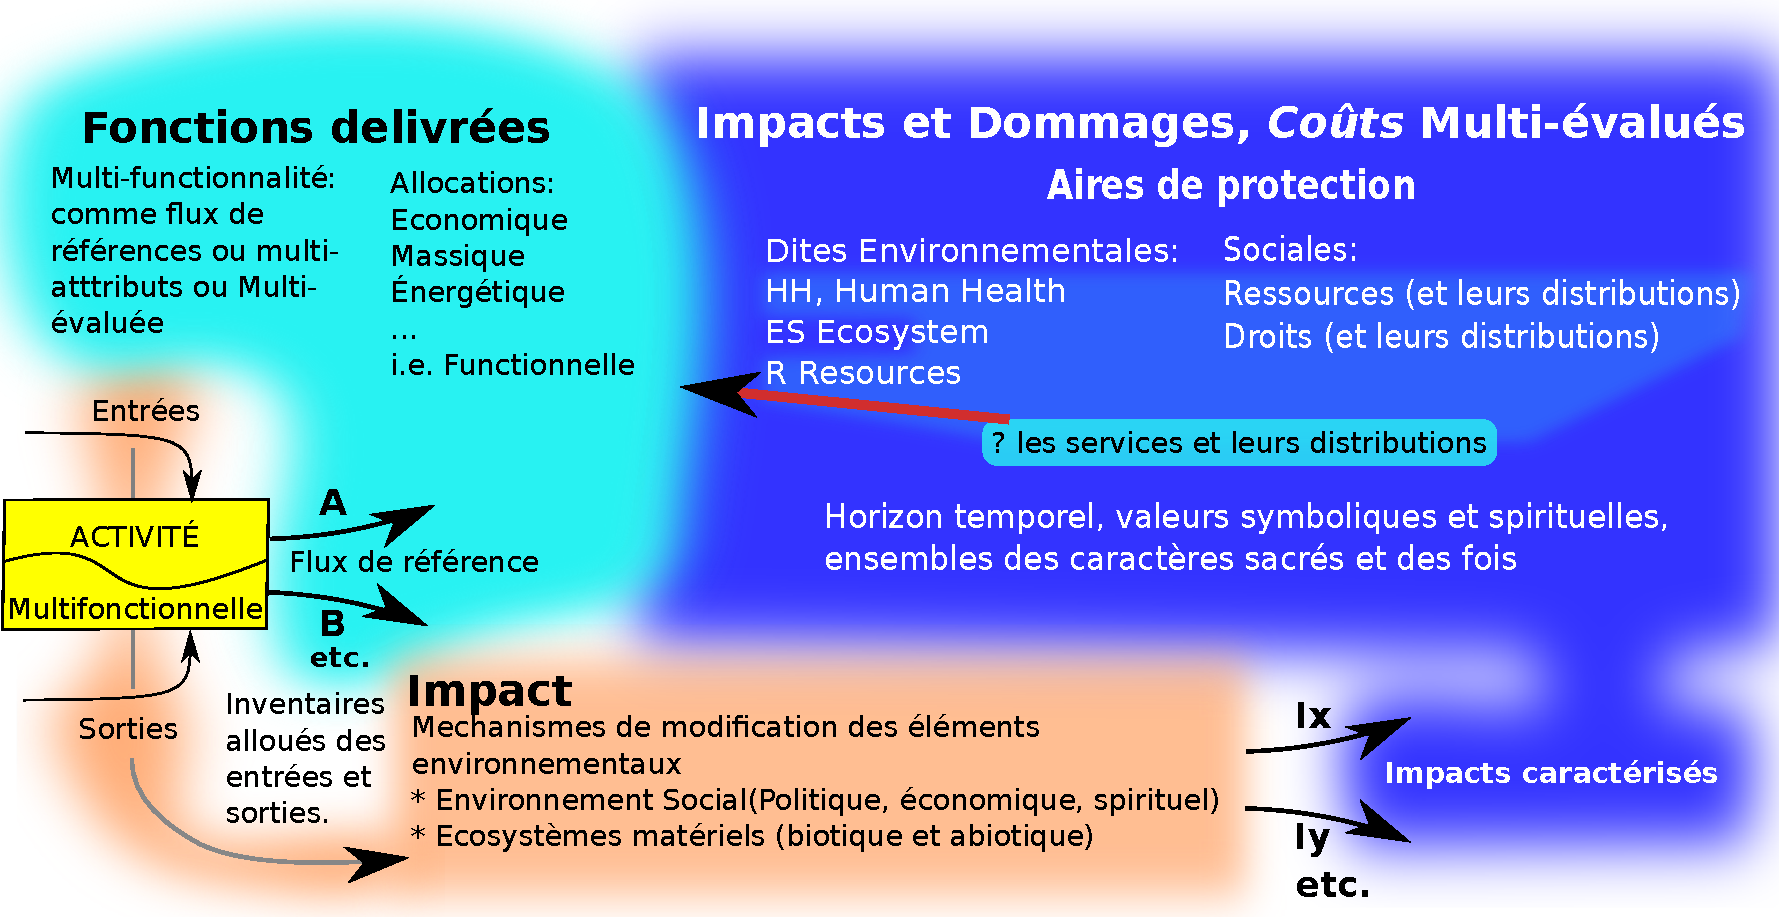
\includegraphics[width=1\textwidth]{/home/rudy/Documents/rudy/01_These/11_production/01_COMMUNICATION/figures/LCA_and_Values_FR.pdf}
%  \caption{We can see here that bringing S-LCA and LCA enabled us to link the domain of access to services to the services delivered (trough functions) to functional unit. And as a whole, the LCA balances values granted to attributes on the range of flows.}
\caption{Unicité des valeurs à l'inventaire et aux impacts.}
  \label{fig:LCA_and_Values}
\end{figure}
%\end{landscape}

\figbox{
Sur la figure~\ref{fig:LCA_and_Values}, nous partons du procédé (jaune), avec l'allocation entre les produits A et B.
Chaque produit, avec sa part d'inventaire et suivant les 'chemins d'impacts', endommagera des entités appréciées (jugé positivement utile), bien qu'apportant sa part fonctionnelle (jugée utile).
Il y a unicité des domaines des impacts et des services.
Ceci est particulièrement identifié sur les indicateurs sociaux et souligné par la flèche rouge relocalisant les services et leur distribution vers les fonctions délivrées.}

%\begin{landscape}
\begin{figure}
%  \textwidth*0.5 : pas fonctionné
%  figure à créer depuis le poster
  \centering
  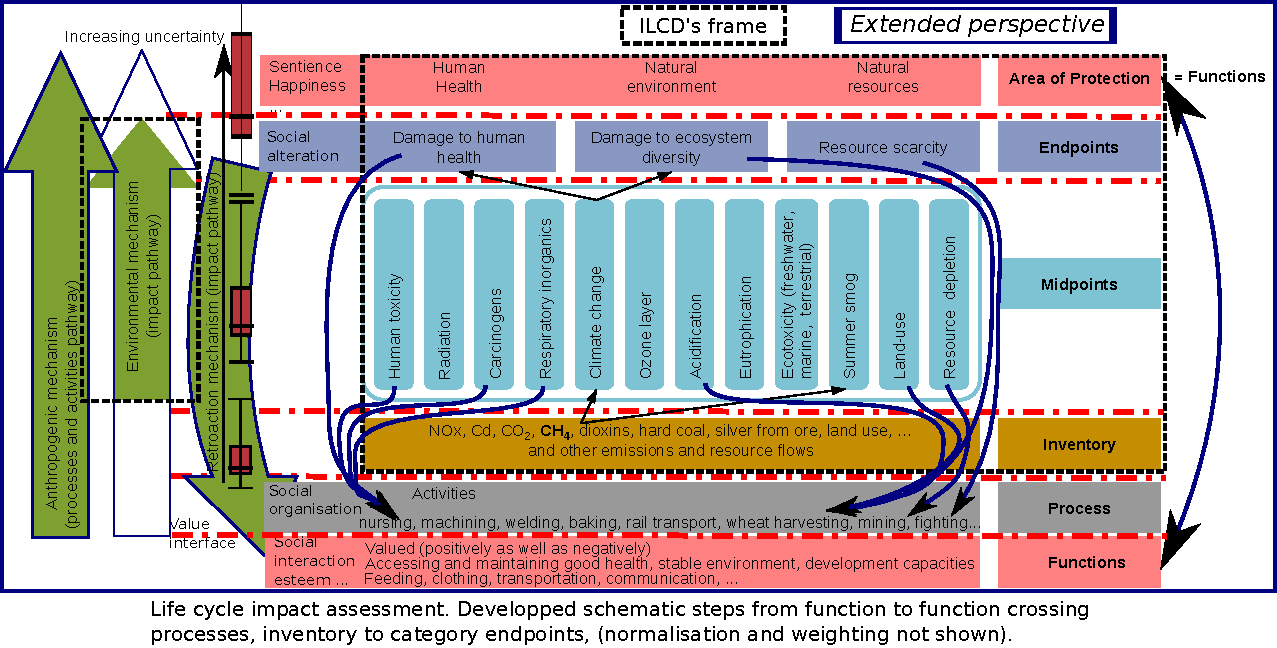
\includegraphics[width=1\textwidth]{/home/rudy/Documents/rudy/01_These/11_production/01_COMMUNICATION/figures/ILCD_LCA_LCIAM_extended_principles.pdf}
%  \caption{We can see here that bringing S-LCA and LCA enabled us to link the domain of access to services to the services delivered (trough functions) to functional unit. And as a whole, the LCA balances values granted to attributes on the range of flows.}
\caption{Représentation alternatives et synthétique de l'unicité des valeurs à l'inventaire et aux impacts.}
  \label{fig:LCA_and_Values2}
\end{figure}
%\end{landscape}

\figbox{
Sur la figure~\ref{fig:LCA_and_Values2}, le cadre de travail classiquement représenté (cadre pointillé) de l'inventaire aux indicateurs endpoint et étendu.
Il faut en fait partir des \emph{fonctions} délivrées par des procédés, des mécanismes, des \textbf{utilités recherchées} \emph{à produire}.
Les flux induits pas ces procédés (l'inventaire) généreront des impacts et des dommages (mid- puis end-point).
Ces dommages sont des dégradations des aires de protection.
Nous avons atteint les \textbf{utilités recherchées} \emph{à maintenir et protéger}.}
%The same issue in defining function, the domain and boundaries to include to complete this function, the allocation and valuation of impacts are the same problem of evaluating multi-valued object.

Il n'y a en fait que l'évaluation d'états différents (social wellfare).
Traiter l'ensemble de la démarche sous l'angle de l'évaluation multidimensionnelle semble en fait rejoindre les travaux de longue date des économistes~\cite{arrow_determination_1952}.
Plus particulièrement, l'angle de traitement de la multifonctionnalité par expansion (sans substitution ni mise à l'échelle) est assez proche de la confrontation de 'panier de biens multiples et hétérogènes' de \citeauthor{arrow_determination_1952} en \citeyear{arrow_determination_1952} avec \citetitle{arrow_determination_1952}.
Nous avons déjà donné une représentation de ceci dans la seconde partie de la figure~\ref{fig:partition_expansion}.

\section{Indicateurs \ldots d'autres méthodes ?}
Dans l'état de l'art, nous avons sommairement survolé la question des méthodes.
Nous ne sommes toutefois pas descendu jusqu'aux mécanismes de constitution des indicateurs.
Nous allons discuter ici le principe de description des mécanismes environnementaux et les indications associés.

En effet, les méthodes d'impacts produisent une indication numérique des impacts ou dommages potentiels sur la base des 'intrants' dans les 'mécanismes environnementaux'.
Poussons la description de l'environnement sur la même direction que les procédés de transformation de la matière.
Nos procédés techniques sont appliqués pour \emph{ajouter} une \emph{valeur}\footnote{Au sens richesse.} à une matière d’œuvre.
Nous jugeons comme dommage une modification d'une aire de protection lui ayant \emph{ôté} une part de \emph{valeur}\footnote{IDEM préc.}.
En fait, nous pourrions modéliser les méthodes d'impacts comme les mécanismes environnementaux dont elles ne seraient que des descriptions.

Une partie \emph{descriptive} n'inclue pas de \emph{jugement}.
Il s'agit donc de poser une description sur laquelle un jugement puisse être appliqué.
Il serait également judicieux de reprendre tout ou partie du langage des experts des domaines concernés.
Prenons des éléments de méthodes d'impacts et traitons les en cas d'exemples.

\subsection{Le cas du vivant}

Deux aires de protection des trois généralement admise porte sur le vivant (santé humaine et vie de l'écosystème)
Partons donc de l'observation des indicateurs sur le vivant.
Les méthodes doivent documenter les modifications que peuvent subir des éléments de l'environnement auxquels nous associons de la valeur sans anticiper cette appréciation ou dépréciation.

Prenons le cas de l'eutrophisation.
La documentation de la méthode ReCiPe 2008~\cite{goedkoop_recipe_2013}, indique concernant l'eutrophisation l'emploi d'autres modélisations (CARMEN :  CAuse effect Relation Model to support Environmental Negotiations, EUTREND).
La source citée mentionne malheureusement un manuscrit non publié~\footnote{Beusen A (2005). User manual of CARMEN1. National Institute of Public Health and Environmental Protection (RIVM), Bilthoven (\textbf{Manuscript, not published})}.
La figure 6.2 du rapport précité, documente la caractérisation en réduction du nombre d'espèces présentes (PDF potentially disappeared fraction).
Le rapport en mentionne un second de 2005 de la STOWA (Stichting Toegepast Onderzoek Waterbeheer, Fondation pour la recherche appliquée sur l'eau), absent dans leurs références.
Sans doute fait-il partie des publications accessibles de la STOWA \ldots \footnote{\href{http://www.stowa.nl/publicaties/publicaties/}{Lien vers les publications de la STOWA.}}

Pour autant, bien que maigre, la documentation a le mérite de faire partie des plus riches qui soient \emph{accessibles}\footnote{À comparer aux autres documentation de méthodes.} et nous permet d'identifier des sources des méthodes d'impacts.
Ainsi nous comprenons qu'une cartographie des concentrations des éléments C,H,O,N,P, ainsi que la documentation des métabolismes de la faune et de la flore, ainsi que de son recensement sur les territoires, permettrait de mettre en œuvre de façon continue la caractérisation de l'environnement.
Nous nous apercevons que la description `objective' est réalisé un pas plus tôt avant l'entrée dans le domaine actuel de l'ACV.
Il faut reculer cette frontière.
Une évaluation holistique opérationnelle doit opérer directement sur le champ objectif.

Puisque nous traitons ici dans ce chapitre des questions de dimensions, soulignons la suivante.
Au delà de la question spatiale, la dimension temporelle est également en jeu ici.
Nous avons traiter de cette dimension au~\ref{subsec:Considérer le temps}.
Le temps intervient dans les questions de toxicologie, tant envers l'homme que tout autre espèce vivante, mais aussi sur l'abiotique.
Les travaux récents sur l'acidification illustrent ce point~\cite{van_zelm_time_2007}.
Chaque indicateur, chaque dimension d'impact et sous l'influence de la dimension temporelle avec des écarts importants dans la caractérisation.
%\footnote{
\blockcquote[traduction]{van_zelm_time_2007}{
Puisque l'emplacement des émissions et des zones forestières sont connus et utilisés comme entrées dans les modèles de 'devenir' (fate of emission), \emph{il serait, en principe, possible de calculer des facteurs de caractérisation régionaux spécifiques pour l'acidification}.
À cet effet, les matrices source-récepteur spécifiques de la substance à un niveau des pays pour les modèles de transport atmosphérique de EUTREND doivent être développés et combinés avec le modèle SMART2.
%Since the location of emissions and forest areas are known and used as input in the fate models, \emph{it would, in principle, be possible to calculate region-specific characterization factors for acidification}. For this purpose, substance-specific source-receptor matrices on a country level for the atmospheric transport model EUTREND need to be developed and combined with the SMART2 model.
}
\keybox{
Toutefois, ce que nous retenons de ce type de travaux n'est pas uniquement la possibilité de calculer des facteurs régionaux spécifiques.
%}.
\textbf{Ce que nous retenons surtout, c'est la possibilité d'observer directement les modèles qui apparaissent dans ces publications (CARMEN, EUTREND, SMART2)}.
Tous ces travaux inaccessibles ou non publiés sont à la base des éléments objectifs pour la rationalisation des décisions.
Et parce qu'ils sont fondamentaux dans la constitution des indicateurs pour la décision, ils doivent être librement accessibles, vérifiables, reproductibles et exploitables.
}

Les travaux de \citeauthor{schmidt_development_2008} indiquent également une relation entre le territoire et sa caractérisation (convergence variable suivant la surface selon les zones caractérisées).
Dans ces travaux, l'horizon temporel choisi peut aussi affecter la prise en compte (ou non) de régénération future (ex : étalement du délai de `re naturalisation' "Renaturalisation time" de l'année à plusieurs milliers d'années)~\cite{schmidt_development_2008}.
Ainsi les inconsistances temporelles ont une forte influence sur le résultat par l'écart observé sur les facteurs d'impacts.

Pourrions-nous \emph{ne pas fixer} un découpage temporel pré-établi (pourquoi pas des horizons temporels à 150, 200, 250 ans)~\barre{?}~!
Laissons les décideurs définir le point de la courbe qui fera valeur pour eux.
Voyons ce point avec la toxicité et l'éco-toxicité et prenons la question sous le cas de l'indicateur \gls{DALY}, développé par \citeauthor{murray_quantifying_1994} dès \citeyear{murray_quantifying_1994}\footnote{\citetitle{murray_quantifying_1994} fut suivi d'autres publications d'explication et de justification~\cite{murray_disability-adjusted_2012,murray_global_1997,murray_evidence-based_1996,murray_quantifying_1994,murray_understanding_1997}. La volonté affichée est la \textbf{quantification objective}, basée sur des \emph{preuves} \citetitle{murray_evidence-based_1996}.}.

Reprenons l'article initial de \citeauthor{murray_quantifying_1994} et détaillons la présentation faite de l'indicateur point par point.
\blockcquote[traduction]{murray_understanding_1997}{
L'unité de mesure en années de vie ajustées sur l'incapacité (disability adjusted life years DALY)
[\dots]
% Utilisé ces dernières années pour quantifier le fardeau des maladies, des blessures et des facteurs de risque sur les populations humaines,
est fondée sur des principes économiques et éthiques convaincants et peut orienter les politiques vers la prestation de soins de santé la plus économiquement-efficace et équitable.
DALY suit un principe d'équité qui traite de manière égale ('like as like') l'ensemble des informations comprenant les conditions de santé des individus, différenciés uniquement par l'âge et le sexe.
Les \emph{poids} particuliers des états de santé utilisés pour tenir compte des résultats des pathologies non létales \emph{sont tirés de l'application de diverses formes de compromis personnels.}
%The measurement unit disability-adjusted life years (DALYs),
%[\ldots]
%%used in recent years to quantify the burden of diseases, injuries and risk factors on human populations,
%is grounded on cogent economic and ethical principles and can guide policies toward delivering more cost-effective and equitable health care.
%DALYs follow from a fairness principle that treats 'like as like' within an information set comprising the health conditions of individuals,
%differentiated solely by age and sex.
%The particular health state weights used to account for non-fatal health outcomes are derived through the application of various forms of the person trade-off.
}
%cogent = convaincant
%\begin{equation}
%\Delta _ {i j}^t  = \int_{a_i^t}^{a_i^t + L(a_i)} KD_jC_{xe}^{-\beta x}e^{-r(x-a_i^t)}dx
%\end{equation}

Nous observons que la seule dimension (et mesure associée) \emph{apparente} dans l'expression du DALY est le temps (une durée, entre deux instants) ($\int_{x0}^{x1}dx$).
Tous les autres éléments sont des applications de jugements~: sur la déficience, l'âge, le futur (actualisation).
Les mesures associées à cela n’apparaissent plus qu’indissociablement mêlées de jugements.
\begin{equation}
\int_{x=a}^{x=a+L} \underbrace{D}_{\substack{\text{pondération}\\ \text{de la}\\\text{déficience}}} \hspace{-0.4cm} \overbrace{Cxe^{-\beta x}}^{\substack{\text{pondération}\\\text{de l'âge}}} \hspace{-0.3cm} \underbrace{e^{-r(x-a)}}_{\substack{\text{décote}\\\text{continue,}\\ \text{'actualisation'}}}dx
\label{eq:DALY}
\end{equation}
Par exemple, pour l'actualisation (dépréciation sur l'avenir sous motif d'incertitude)~: \blockcquote[traduction]{murray_quantifying_1994}{
Reconnaissant que le débat sur l'actualisation des bénéfices pour la santé ne sera pas résolu dans un proche avenir, \textbf{nous avons choisi un taux positif faible de 3 pour-cent} pour le calcul des DALYs.
%Recognizing that the debate on discounting health benefits will not be resolved in the near future, \textbf{we have chosen a low positive rate of 3 percent} for the calculation of DALYs.
}

Donc le DALY est l'unité d'un indicateur (pas juste d'une simple mesure) qui dépend du sexe et de l'âge (comme indiqué explicitement dans l'article), mais aussi, de la population de référence choisie pour les espérances de vie, de l'appréciation de la pathologie par celle-ci, de l'appréciation variée du temps durant une vie par celle-ci.
Enfin à supposé que l'ensemble des jugements sur chaque domaine soit bien issue d'une même population et non pas partiellement accaparé par des 'experts'.

Évidement d'autres mesures alimentent ces jugements (mesures biomédicales pour la détermination de la pathologies et l'emploi de la pondération respective par exemple).
Mais l'on constate que les jugements de valeurs sont très imbriqués (comme dans toute forme d'agrégation d'informations incommensurables).

\figbox{
Dans un article ultérieur~\cite{murray_understanding_1997}, \citeauthor{murray_understanding_1997} détaillent~:
\begin{equation}
\Delta_{ij}^{t} = \int_{x=a_i^t}^{x=a_i^t+L(a_i)} KD_jCxe^{-\beta x}{e^{-r(x-a_i^t)}}dx
\label{eq:DALY-97}
\end{equation}
\begin{align}
DALYs[r,K]
& = D
\left\{
 \frac {KCe^{r a}}{(\beta + r)^2}\big[e^{-(\beta + r)(L+a)}[-(\beta + r)(L+a)-1] \right.\nonumber\\
& \qquad \left. - e^{-(\beta + r)a}[-(\beta + r)a-1]\big] \frac {1-K}{r}(1-e^{rL}) \right \}
\end{align}
\blockcquote[traduction]{murray_understanding_1997}{
Où x est le temps, a est l'âge d'apparition, Dj est un poids d'invalidité due à la séquelle j.
D est de 0 pour la santé parfaite, avec les pires conditions d'invalidité il approche 1;
la mort se voit attribué une valeur de 1.
D ne constitue pas une mesure absolue; il a au moins des propriétés d'échelle d'intervalle.
Éq. (1) permet la possibilité qu'à chaque année de vie peut être attribué un poids non uniforme:
C est la constante de correction de pondération de l'âge ;
et $ \ beta $ est le paramètre de pondération de l'âge telle que le poids maximum pour une année de vie à un âge donnée est affectée à ($ 1 / \ beta $).
r est le taux de réduction, a est l'âge actuel;
L (a) est la durée de l'état dans le cas d'un handicap ou l'espérance de vie normale à l'âge a '; dans les cas mortel.
K est un paramètre, soit 0, soit 1, et fonctionne en tant que facteur de modulation de la pondération de l'âge.
%where x is time, a is the age of onset, Dj is a disability weight due to sequela j.
%D is 0 for perfect health with the worst disability condition approaching 1 ; death is
%assigned a value of 1.
%D is not an absolute measure; it has at least interval scale properties.4
%Eq. (1) allows the possibility that each year of life can be assigned a non-uniform weight: C is the age-weighting correction constant; 5
%and $\beta$ is the age-weighting parameter such that the peak weight for a year of life is assigned at
%age ($1/\beta$).
%r is the rate of discount, a~ is the current age;
%L(a) is the duration of the condition in the case of disabilities or the standard life expectancy at age a'; in the case of death. 6
%K is a parameter, either 0 or 1, and functions as the age weighting modulation factor.
}
%\begin{equation}
%- \Bigg[ \frac {DCe^{-\beta a}}{(\beta + r)^2}[e^{-(\beta + r)(L)}(1+(\beta + r)(L+a))-(1+(\beta + r)a)]\Bigg]
%\end{equation}
%\begin{equation}

%\end{equation}
}
Le nombre de \emph{poids} (weight) discuté dans les détails de Eq.~\eqref{eq:DALY-97} souligne à lui seul la subjectivité de l'outil.
Alors, nous pouvons nous demander si la volonté affichée d'un traitement 'égalitaire' comme si celui-ci était 'neutre' ('like as like') n'est pas qu'un signe de notre incapacité à gérer explicitement l'intégration du jugement de valeurs en situation réelle ?
La réalité et la multi-dimensionnalité attenante impliquée, soulignent l'incommensurabilité des informations observées~: \barre{'like as like'},'nothing is alike' !

Nous pouvons donc interroger la perception du décisionnaire sur ce type d'indicateur agrégé.
Quelle serait la propre hiérarchisation du décideur sur la pondération des pathologies par exemples~?
\exbox{
L'infertilité est relativement très faiblement pondérée.
\blockcquote[extrait et traduction de la pondération]{salomon_common_2012}{
Infertilité: primaire 0·011 (0·005–0·021)\\
Infertilité: secondaire 0·006 (0·002–0·013)\\
Brûlures de moins de 20\% de la surface totale sans brûlures des voies aériennes basses~: court termes, avec ou sans traitement 0·096 (0·062–0·140)
%total surface area without lower airway burns: short term, with or without treatment 0·096 (0·062–0·140)
}
Nous observons les indicateurs sur la santé de l'éco-système avec la diversité des espèces et les menaces à cette diversité (extinction).
Questionnons nous la perspective individualiste du traitement de la santé humaine~\footnote{ex. dans ReCiPe.
'birth' : 1 occurrence ;
'reprotoxic' : 0 occurrence.)}~?
}
Nous observons pour notre espèce, la dégradation de la santé d'une population vivante.
Nous sommes nettement moins attentif aux obstacles à la reproduction des espèces (M-R des CMR), soit la dégradation des populations futures, même pour notre propre espèce.


Sur le \emph{principe de pré-évaluation} tel que présent dans les méthodes d'impacts actuellement implémentées, nous observons un nombre de choix inclus et mêlés aux observations.
C'est dans l'ouverture de ces jugements qu'il convient de chercher d'\emph{autres} méthodes.
À ce titre, il est important de reprendre l'analyse dimensionnelle des objets manipulés.

\section{Interprétation}
L'interprétation est itérativement sollicitée à chacune des trois autres étapes de l'ACV (but et périmètre ; inventaire ; caractérisation).
Toutefois, bien que nécessaire à toute forme d'interprétation, la déclaration des jugements dans les études est généralement absente.
Cela est d'autant plus surprenant que la question 

!!! pb ref finnveden

%(\citetitle{finnveden_valuation_1997}~\cite{finnveden_valuation_1997}) 
est présente depuis les années 90~\cite{freidberg_behind_2015} et donc depuis la période d'élaboration des ISO, de leurs initiations jusqu'aux dernières révisions
~\cite{volkwein_valuation_1996,hertwich_decision-analytic_2001,hofstetter_value_2002}.
%~\cite{volkwein_valuation_1996,finnveden_valuation_1997,hertwich_decision-analytic_2001,hofstetter_value_2002}.
\blockcquote[traduction]{hertwich_decision-analytic_2001}{
Le débat sur les valeurs qui a été déclenchée par le groupe de travail sur les méthodes d'impact de l'ACV de la \gls{SETAC} Amérique du Nord (OWENS et al., 1997) et la norme ISO 14042 sur l'évaluation des impacts en ACV de l'Organisation Internationale de Normalisation qui nous a incité à l'examen du raisonnement dans l'ACV.
Qu'est-ce que l'ACV~?
Comment peut-il être justifié~?
Sur quels arguments peut être basé le choix des méthodes~?
Comment peut-on distinguer les bonnes méthodes de mauvaises méthodes, les déclarations valides des non valides~?
Ce projet nous a d'abord conduit à développer une base théorique, philosophique LCA (HERTWICH et al., 2000).
Notre conclusion principale est que l'ACV peut être justifiée par son utilisation dans la prise de décision.
%The values debate that was triggered by the working group
%on LCA impact assessment of the Society of Environmental
%Toxicology and Chemistry (SETAC) North America (OwENs
%et al., 1997) and the International Standard Organization's
%ISO 14042 standard on LCA impact assessment prompted
%us to investigate the reasoning in LCA. What is LCA? How
%can it be justified? What can arguments about method choice
%be based on? How can we distinguish good methods from
%bad methods, valid from invalid statements? This project lead
%us to first develop a theoretical, philosophical foundation of
%LCA (HERTW~CH et al., 2000). Our central conclusion was that
%LCA can be justified by its use in decision making.}
}

Il semble donc que l'avertissement de \citeauthor{hertwich_theoretical_2000} n'est pas été suivi~\cite{hertwich_theoretical_2000}.
Rappelons le ici.
\blockcquote[traduction]{hertwich_theoretical_2000}{
Hertwich \& Pease expriment la préoccupation que le document 14042 impose des contraintes et des limitations extrêmes sur l'ACV et l'AICV\footnote{Plus rarement employé en français, LCIA, évaluation des impacts du cycle de vie.}, en particulier pour le cas des assertions comparatives. Ils caractérisent le langage utilisé dans le projet du comité comme étant biaisée vers les sciences naturelles et \emph{accusent le comité d'ignorer les perspectives et idées des disciplines académiques qui traitent des questions de valeur}.
%Hertwich \& Pease express the concern that the 14042 document imposes extreme constraints and limitations on LCA and LCIA, especially for the case of comparative assertions. They characterize the language used in the committee draft as being natural science biased and accuse the committee of ignoring insights from academic disciplines that address value questions.
}
La méthodologie ne fait aujourd'hui encore apparaître aucun compartiment pour recueillir l'ensemble des jugements qui constellent la méthode.
Lorsque certains jugements sont décrits (pondération, allocation, indicateurs), il n'y a pas de justification sur ces choix relativement aux parties prenantes identifiées comme décideur.

Certains points de jugements sont traités en méthode d'impacts.
Tels furent les travaux autour de la construction de "Eco-indicator 98" avec la pondération par panel sur la base de trois "système de valeurs" basés sur la 'Théorie Culturelle'(Cultural Theory (Mettier, 1999)) citant (Hofstetter, 1998))

!!! pb ref finnveden

%\cite[p.~36]{finnveden_critical_1999}.

Ce principe se retrouve aujourd'hui dans les méthodes déclinant leurs facteurs suivant des perspectives, individualiste (I), hiérarchiste (H) ou égalitariste (E)~\cite{goedkoop_recipe_2013}.
Les praticiens sont malheureusement tributaires des archétypes choisis, comme de la façon dont ils sont implémentés dans les méthodes d'impacts.
La cohérence des jugements sur l'ensemble de la méthodologie est d'autant plus difficile à obtenir que la littérature sur les méthodes d'impacts n'isole pas les jugements qu'elles intègrent dans ses archétypes dans un compartiment repérable et ré-exploitable.
C'est à dire qu'il n'est pas possible actuellement de faire correspondre de façon consistante les jugements dans les méthodes d'impacts à ceux du décideurs.

D'autres éléments de jugement (d'interprétation) quasi-systématiquement présents dans les outils de modélisation et caractérisation servant l'interprétation finale, se situent dans la \emph{normalisation}.
Une présence d'autant plus surprenante que cette pratique n'apporte pas d'éléments à l'interprétation sinon qu'\emph{un biais conservateur}
%La problématique de la normalisation est renforcée avec le PEF.
et \emph{une erreur dimensionnelle}.

Toutes les références mentionnent la normalisation.
\begin{description}
\item \textbf{ILCD}~:
\blockcquote[traduction, p 275. 8.1 Introduction and overview (Refers to aspects of ISO 14044:2006 chapter 4.4.1, 4.4.2, and 4.4.3)]{european_commission_ilcd_2010}{
Dans une étape \textbf{facultative} ultérieure, les résultats de l'AICV peuvent être multipliées par des facteurs de normalisation qui représentent l'inventaire global d'une référence (par exemple tout un pays ou un citoyen moyen), ce qui produit des résultats d'AICV normalisés \textbf{sans dimension} (8.3).
%In a subsequent, optional step, the LCIA results can be multiplied with normalisation factors that represent the overall inventory of a reference (e.g. a whole country or an average citizen), obtaining \textbf{dimensionless}, normalised LCIA results (8.3).
}
\item Dans le \textbf{Official Journal of the European Union}\footnote{L 124/1
RECOMMENDATIONS COMMISSION RECOMMENDATION of 9 April 2013 on the use of common methods to measure and communicate the life cycle environmental performance of products and organisations (2013/179/EU)}, qui y fait appel également,
nous soulignerons cependant quelques mots qui ont toute leur \emph{importance}.
\blockcquote[traduction]{commission_europeenne_commission_2013}{
Normalisation - Après l'étape de caractérisation, la normalisation est une étape \textbf{facultative} dans laquelle les résultats de l'évaluation de l'impact EF [environmental footprint] sont multipliés par les facteurs de normalisation qui représentent l'inventaire global d'une unité de référence (par exemple un pays entier ou un citoyen moyen).
Les résultats normalisés de l'évaluation des impacts expriment les parts relatives des impacts du système analysé en termes de total des contributions à chaque catégorie d'impact par unité de référence.
Lors de l'affichage des résultats d'évaluation de l'impact normalisés des différents sujets d'impact les uns à côté des, il devient évident de dire quelles sont les catégories d'impact les plus, et moins, touchées par le système analysé.
Les résultats de l'évaluation de l'impact normalisés \underline{ne} \underline{reflètent} \underline{que} \underline{la} \underline{contribution} du système analysé au potentiel d'impact total, \underline{pas} \underline{la} \underline{gravité} / la \underline{pertinence} \underline{du} \underline{total} \underline{respectif} \underline{de} \underline{l'impact.}
Les résultats normalisés sont \textbf{sans dimension}, mais pas d'additif.
%Normalisation – After the characterisation step, normalisation is an optional step in which the EF impact assessment results are multiplied by normalisation factors that represent the overall inventory of a reference unit (e.g. a whole country or an average citizen).
%Normalised EF impact assessment results express the relative shares of the impacts of the analysed system in terms of the total contributions to each impact category per reference unit.
%When displaying the normalised EF impact assessment results of the different impact topics next to each other, it becomes evident which impact categories are affected most and least by the analysed system.
%Normalised EF impact assessment results \underline{reflect only the contribution} of the analysed system to the total impact potential, \underline{not} \underline{the} \underline{severity}/relevance \underline{of the respective total} \underline{impact.}
%Normalised results are \textbf{dimensionless}, but not additive.
}
\item \textbf{PEF}~:
\blockcquote[traduction, 6.2.1 Normalisation of Environmental Footprint Impact
Assessment Results (\underline{\textbf{recommended}})]{commission_europeenne_commission_2013}{
Par conséquent, des résultats normalisés \textbf{sans dimension} sont obtenus.
%As a result, \textbf{dimensionless} normalised OEF results are obtained.
}.
\end{description}


PRIMO, il n'y a pas a-dimensionnement par la méthode décrite mais homogénéité dimensionnelle.
Il semble que la communauté de notre discipline oublie la division qu'elle a placé au centre de la méthodologie.
\blockcquote[traduction, 7.4.2.6 Reference amount of the reference flow (Refers to aspects of ISO 14044:2006 chapter 4.3.3]{european_commission_ilcd_2010}{
Les données individuelles pour l'inventaire doivent chacun être quantitativement exprimés en flux \underline{\textbf{par unité fonctionnelle}}.
%The individual data for the inventory must each be quantitatively expressed as flows per
%functional unit.
}
Partant d'une base d'impact d'un service (\gls{UF}), la normalisation consiste en la division par une référence (sous deux formes, interne ou externe).
Concernant les formes internes, il s'agit de déterminer le composant ou le procédé (élément local) qui contribue aux indicateurs dans la globalité du service observé (cycle de vie du système principal étudié).
\begin{equation}
%$
\frac{\barre{\text{Unité~d'impact}} / \text{Sous-Unité~fonctionnelle~locale}}
{\barre{\text{Unité~d'impact}} / \text{Unité~fonctionnelle~globale}}
%$
\end{equation}
Les références externes sont généralement des populations prises sur une durée d'un an.
\begin{equation}
%$
\frac{\barre{\text{Unité~d'impact}} / \text{Unité~fonctionnelle}}
{\barre{\text{Unité~d'impact}} / \text{(pers/année)}}
%$
\end{equation}

Les erreurs de dimension sont reprises dans les tables des facteurs de références.
\begin{figure}[htbp]
\centering
\includegraphics[width=0.9\linewidth]{/home/rudy/Documents/rudy/01_These/11_production/01_COMMUNICATION/figures_extraites/JRC/JRC_Normalisation_facteur_EU27_2010.pdf}
\caption{Erreurs sur les facteurs de normalisation (JRC, EU27-2010).}
\label{fig:facteurs de normalisation EU27-2010}
\end{figure}
\figbox{
Nous soulignons en rouge dans la table 'commentée' du rapport du JRC, figure~\ref{fig:facteurs de normalisation EU27-2010}, les incohérences dimensionnelles.

Il apparaît comme évident que les impacts de référence sont établis par an (2010), par personne (avec soit le total des 27 pays de l'union européenne ou un pseudo européen moyen).
}

Nous pourrions débattre plus longtemps de l'influence des bases normatives sur les résultats d'évaluation, dont 
\citeauthor{kim_importance_2013} ont conclu à l'\emph{importance décisive}~\cite{kim_importance_2013}.

La revue du traitement de la normalisation est faite par \citeauthor{finnveden_recent_2009}\cite{finnveden_recent_2009}.
\blockcquote[traduction]{finnveden_recent_2009}{
Pour la normalisation, les développements ont été réalisés en ce qui concerne la collecte de données plus exactes, à jour, et complètes pour différentes régions (Stranddorf et al., 2005; Bare et al., 2006; Lundie et al, 2007b;. Wegener Sleeswijk et al., 2008) ainsi que des choix liées à la méthode.
Par exemple, dans une base de données de normalisation nationale, les émissions du pays devraient-elles être incluses en tant que telles, ou devraient-ils être corrigés pour l'importation et l'exportation, ou même pour le décalage temporel entre la production et l'émission, comme dans les équipements électriques qui seront mis au rebut seulement 20 ans après (Wegener Sleeswijk et al., 2008)?
Un autre exemple de développement lié à la méthode est la reconnaissance du fait que les données manquantes peuvent introduire un biais plus compliqué pour un score normalisé que pour un score non normalisé (Heijungs et al., 2007).
%For normalisation, developments have been made with respect to more accurate, up-to-date, and complete data collection for different regions (Stranddorf et al., 2005; Bare et al., 2006; Lundie et al., 2007b; Wegener Sleeswijk et al., 2008) as well as to some method-related choices.
%For instance, should in a national normalisation database the emissions of the country be included as such, or should they be corrected for import and export, or even for time-lags between production and emission, as in electric equipment that will be discarded only 20 years afterwards (Wegener Sleeswijk et al., 2008)?
%Another example of a method-related development is the recognition that data gaps can introduce a more complicated bias for a normalized score than for an unnormalized score (Heijungs et al., 2007).
}

Toutefois cette pratique dans sa conception actuelle est sans intérêt de soutenabilité.
Chose qui étonnamment est passée sans commentaire antérieur spécifique à la chose.
Nous y passons donc avec le point suivant.


SECUNDO, \textit{Normal} ne signifie pas \textit{Soutenable}.
Ceci est d'autant plus vrai que nous ne disserterions pas du sujet si notre \emph{normalité} n'était pas actuellement \emph{insoutenable}.
S'il est employé dans les mécanismes évaluatifs pour la prise de décision, ce mécanisme n'a qu'un \emph{caractère conservateur} des tendances actuelles.
\exbox{
Partez d'un set d'impacts générés par une population X.
Nous prendrons volontairement de faux indicateurs.
Disons 'émission de A, agent mortel' émis en grande quantité (100.000 unités) et 'B une substance modérément irritante' émise dans des quantités modérées ou faibles (100 unités).
Lorsque vous 'normaliserez', l'inventaire du produit ou service observé sera \emph{divisé} par votre référence (100.000A/(an~.~population X) ; 100B/(an~.~population X)).

Si un service émet anormalement plus de B (disons 1B), mais toujours en émettant du A (10A), B face à A ressortira dans l'histogramme des ratios d'indicateur homogène en dimension en $\frac
{\mathit{(pers.année)}}{\mathit{Unité~fonctionnelle}}$ (1/100 face à 1/10.000).
Vous vous concentrerez alors sur un aspect modérément irritant au lieu d'un danger mortel, simplement parce qu'il est `anormal' selon votre référence.

En vous concentrant sur l'action de réduire ce qui sort de la norme, vous maintenez la norme.
\textbf{La normalisation est un principe conservateur.}
}
L'évolution d'une mention \emph{optionnelle}, \emph{facultative}, dans les documents antérieurs à une recommandation (dans la méthodologie du PEF), nous semble donc particulièrement inadéquate voir dangereuse.

La seule utilité potentielle dans les références d'émissions consisterait à son emploi dans une pratique de \emph{distance à la cible} où, en plus d'une priorisation des indicateurs, les références serviraient à prioriser l'action face à un écart de la situation actuelle face à la situation souhaitée.

Ces outils sont à surveiller avec attention.
En effet, une orientation instrumentaliste peut tout à fait avoir un caractère conservateur opposé à ce qui serait considéré comme un progrès environnemental comme cela a déjà été décrit par \citeauthor{finnveden_limitations_2000}.
\blockcquote[traduction]{finnveden_limitations_2000}{
La simple utilisation de l'ACV ne conduira cependant pas à des impacts environnementaux réduits.
Comme indiqué plus haut, l'ACV peut être utilisée comme un outil conservateur pour faire obstacle aux modifications qui seraient bénéfiques pour l'environnement.
%The mere use of LCA will however not lead to reduced environmental impacts. As discussed above, LCA can be used as a conservative tool to obstruct changes that would be environmentally beneficial.
}\footnote{Nous rejetons qu'il existe un `bénéfice pour l'environnement'.
Cela suppose une personnification de l'environnement et d'une capacité pour lui d'émettre un jugement sur ce qu'il préfère et donc juger d'une satisfaction de sa préférence (un bénéfice).
Toutefois et comme re-démontré, toute évaluation si elle s'applique des principes de normalisation avec une référence à l'antériorité est conservatrice.}

Pour conclure sur la question des références normatives, relevons la contribution suivante.
\blockcquote[traduction, termes personnellement soulignés]{klopffer_subjective_1998}{
La deuxième remarque à propos de la subjectivité que je voudrais faire concerne l'existence de valeurs normatives [2].
Ces valeurs, bien sûr, ne sont pas objectives soit, mais la plupart d'entre elles sont codifiées en quelque sorte.
\underline{Le rang le plus élevé} parmi ces valeurs est donnée par une codification des Nations Unies, par exemple dans la \gls{DUDH}.
Ces valeurs sont contraignantes pour tous les pays membres des Nations Unies, sans aucune exception.
Les règles dérivées de ces valeurs normatives sont subjectives dans le sens indiqué ci-dessus, mais il serait stupide de les attribuer à la nature de l'arbitraire et de la subjectivité individuelle qui semble être la grande peur dans certaines parties de la communauté de l'\gls{ACV}.
Il n'y a pas de doute que ces valeurs normatives et règles \underline{devraient} \underline{être} \underline{utilisées} pour l'évaluation des enjeux mondiaux.
Pour les questions régionales et nationales, les valeurs spécifiques d'une communauté d'États ou d'une seule nation \underline{pourraient} \underline{être} \underline{consultées}.
}
Il convient à ce stade de rappeler que les droits des nations et donc des nations unies, ne sont pas les productions des peuples de ces nations mais de leurs gouvernements.
Une critique de la \gls{DUDH} est faite par \citeauthor{eberhard_au-a_2009}, qui propose des pistes de dépassement de l’approche \emph{universaliste} par un \emph{pluralisme}~\cite{eberhard_au-a_2009}.
\citeauthor{klopffer_subjective_1998} pose une hiérarchie (le rang le plus élevé) et emploie le verbe modal du \textsc{devoir} pour l'usage et le respect de ces codes établis et un modal de \textsc{possibilité} pour une \emph{consultation} de \textit{sous-entités} aux nations unies.

\citeauthor{klopffer_subjective_1998} poursuit~:
\blockcquote[traduction, termes personnellement soulignés]{klopffer_subjective_1998}{
Ceci étant dit, nous devons admettre que l'opérationnalisation des valeurs normatives (\textit{the} normative values) dans des règles simples, \underline{comme} \underline{requis} \underline{par} \underline{l'\gls{ACV}}, est un travail difficile, mais il devrait être possible.
}
C'est ici encore le lexique de l'obligation, quasi naturelle, pour une intégration systémique (règles simples requises).

L'argumentaire de \citeauthor{klopffer_subjective_1998} continu sur une logique d'exemple et généralisation en combinaison avec argument d'autorité scientifique.
\blockcquote[traduction, termes personnellement soulignés]{klopffer_subjective_1998}{
La \underline{manière} \underline{générale} d'obtenir un accord sur les questions qui ne peuvent être résolus de manière objective est la création de conventions.
Un \underline{excellent exemple} dans le monde \underline{scientifique} et technique sont les unités de mesure.
Le système métrique dans sa forme actuelle, le "Système international d'unités" (SI) selon la norme ISO 1000 n'est pas plus scientifique que les autres systèmes bien développés, il est seulement plus cohérente, logique et plus facile à utiliser; et il est le résultat d'un débat international qui a eu cours durant deux siècles.
%The second remark about subjectivity I would like to make concerns the existence of normative values [2].
%These values, of course, are not objective either, but most of them are codified in some way.
%The highest rank among these values is given by a codification by the United Nations, e.g. in the Universal Declaration of Human Rights.
%These values are binding for all member countries of the United Nations without any exception.
%The rules derived from these normative values are subjective in the meaning discussed above, but it would be foolish to attribute them to the kind of arbitrariness and individual subjectivity which seems to be the great fear in parts of the LCA community.
%There is no \emph{doubt} that these normative values and rules \emph{should be used} for valuating global issues.
%For regional and national issues, the specific values of a community of states or of a single nation \emph{may be consulted}.
%
%\textbf{This being said, we have to admit that the operationalization of \emph{the} normative values into simple \emph{rules}, as \emph{required by LCA}, is hard work, but it should be possible.
%The general manner of obtaining agreement on questions which cannot be solved objectively is the creation of conventions.
%An excellent example in the scientific and technical world are the units of measurement.
%The metric system in its present form, the "Système International d'Unités" (SI) according to ISO 1000 is not more scientific than other well developed systems, it is only more consistent, logical and easier to use; and it is the result of an international discussion which has been going on for two centuries.
}

Il y a une confusion entre système de mesures et système de valeurs.
Il faudrait pour accepter cet argumentaire pouvoir faire la généralisation du processus pour obtenir le premier (système métrique) au second (système de valeurs universelles).
La déclaration est d'ailleurs maladroite dans ce qu'elle sépare scientifique et logique (pas plus scientifique, plus logique).
Mais ce n'est pas l'erreur la plus critique.
Le choix des unités de mesures n'est pas équivalent au choix e tà l'arbitrage des valeurs.
Au delà de la commune question dimensionnelle, il faut pour traiter le système de valeurs s'occuper de l'orientation de la préférence et de ses variations.
Si nous posons ces éléments successivement nous obtenons~:
\begin{enumerate}[label=\roman*]
\item le choix de l'unité mesure sur la dimension (facteur d'échelle et origine) pour la compréhension des personnes questionnées~\footnote{
Il faut comprendre ici qu'il n'y a pas de différence à préférer un objet de 2,54 centimètres ou de 1 pouce.
Mais selon l'unité choisie des biais peuvent apparaître lors de l'expression des préférences.
}
\item la définition des préférences internes à une même dimension dans ses orientations, ses formes et son incertitude dans un même contexte 
\item la définition des préférences externes, par paires pour l'ensemble des dimensions.
\end{enumerate} 
Si nous pouvons généraliser au (i), ce qui signifierait l'emploi du système international dans l'ACV, les points (ii) et (iii) sont d'une tout autre nature.
\exbox{
Pour reprendre l'exemple de la température, la préférence pour les boissons chaudes comporte d'abord un premier seuil d'intolérabilité puis une préférence croissante, puis, au delà de la position individuellement préférée, décroissance et enfin second seuil d’intolérabilité.
À quoi s'ajoute évidement la préférence externe aux autres dimensions (amertume, sucrée, apport calorique, odeur\ldots).

Le choix de l'unité n'intervient même pas dans la 'quantification pour le choix'\footnote{Hors biais des unités et de leurs échelles.}.
}

Ainsi les significativités d'un système d'unités de mesures et d'un système de valeurs sont tout à fait différentes.
Ceci induit une critique forte du qualificatif \emph{\textbf{requis}} quant à \textbf{l'opérationnalisation d'\emph{\underline{un}} système normatif de valeurs universelles traduit en règles simples}.

Nous ne disons pas que \emph{des} normes de valeurs ne sont pas \emph{possibles} (elles existent d'ailleurs, sans être explicitées).
De telles normes nous semblent d'ailleurs également nécessaires pour les décisions \emph{collectives}.
Les échelons locaux, nationaux, supra-nationaux et global font également sens pour des décisions à chacune de ces échelles.
Nous ne voyons cependant aucunement pourquoi elles \emph{devraient} être traduites en \emph{règles}, encore moins avec un article définit (the).
Nous soulignons qu'un tel mécanisme aurait également un caractère conservateur.
La subordination et la hiérarchisation préalable à des déclarations antérieures, telle la \gls{DUDH} dans la citation choisie, doit donc être surveillée.

Il en résulte que dans son état actuel l'ACV ne propose aucune assistance à l'interprétation autre que des outils conservateurs manifestement en opposition à la logique d'une soutenabilité en rupture de notre in-soutenabilité actuelle.
Les composants donnés en fin du chapitre~\ref{chap:ACV, la (re)conception d'un outil} répondent à ce manque.
Le compartiment pour les jugements et opinions du point~\ref{sec:Un nouveau standard} est donc un élément central.

\section{Expérimentation}
\begin{center}
\colorbox{yellow}{exp AHP + electre ou promethee depuis données collectées par requêtes SPARQL 1.0 d'abord, fédéré 1.1 ensuite.}
\exbox{reprendre le travail sur enipedia}
\end{center}
\section{Conclusion sur la multidimensionnalité}

La discipline n'a porté que peu d'attention aux problèmes dimensionnelles.
%En atteste les erreurs manifestes de l'ISO, de l'ILCD et autres références de la méthodologie.
La reconnaissance de l'incommensurabilité résout en chaîne la quasi totalité des problèmes non-résolus sur le plan méthodologique.

\begin{itemize}
\item La détermination des convergences en lieu et place des troncatures;
\item l'approche taxonomique multi-échelle des mécanismes environnementaux pour l'abandon des agrégations observations-jugements des `méthodes d'impacts' actuelles;
\item la libre détermination des indicateurs suivis, consistante au système de valeurs décideur en substitut au `package d'impacts' recommandés;
\item l'analyse dimensionnelle systématique;
\item le traitement, avec assistance de techniques d'\gls{ADMC}, en un lieu unique de l'architecture axiologique du décideur pour un traitement consistant sur la globalité de l'évaluation.
\end{itemize}

Voici par cette énumération la prescription pour soigner douze\footnote{
Nous considérons l'aspect `dynamique de l'environnement' dans sa problématique dimensionnelle comme rattaché à l'horizon temporel.
Les problèmes de concentrations dynamiques sont associés au spécificité de l'environnement et au méthodes d'impacts.
Et nous ne le conservons donc que dans la problématique de disponibilité des données.
} maux des quinze dont souffre la méthodologie.

La résolution conjointe, de la multi-dimensionnalité et de la multi-fonctionnalité nous conduit à considérer avec plus de conviction l'approche globale par expansion pure.
Il s'agit dans ce cas de maintenir le caractère fondamental de la pensée en cycle de vie quant au report d'impact et d'accepter renonciation à l'unicité de l'unité fonctionnelle.

La réalisation que `le cycle' qui servait plus à l'illustration méthodologique, pour parcourir l'ensemble de la chaîne de valeur, nous pousserait même à abandonner le terme complètement.
La \emph{pensée en cycle de vie} ne semble n'avoir existé que pour complété les racines de l'\emph{évaluation holistique opérationnelle}.
Sur la base actuelle du développement des réseaux de connaissances sémantiques, avec la prise en compte du jugement du décideur et disposant des nouvelles capacité de requêtes sur ces \textit{nouvelles} bases de données, il semble que la \textbf{modélisation par agents} sera sa modalité principale, la seule que nous puissions envisager à leur actuelle pour sa mise en œuvre.

Ne reste que pour résoudre ainsi \emph{de façon pratique}, les douze premiers item et les deux en complément relatif à la disponibilité des données, il faut traiter la question de l'alimentation de la base de connaissance.
C'est tout l'objet du chapitre suivant.